\documentclass{beamer}
\usepackage{amsmath}
\usepackage{indentfirst}
\usepackage{graphicx}
\usepackage{varwidth}
\usepackage[square]{natbib}
\hypersetup{pdfpagemode=FullScreen}
%\setbeamercolor{background canvas}{bg=}
\usepackage{subcaption}
\usepackage{caption}
\usepackage{hyperref}
%\usetheme{Berlin}
\usecolortheme{beaver}
%\usecolortheme[named=gray]{structure}
%\setbeamercolor{titlelike}{parent=structure,bg=cyan}
\title{Rothermel vs. Balbi rate of spread model}
\subtitle{By: Jeremy Benik}

%\usetheme{lucid}
\begin{document}

\pagecolor{yellow!30!orange}
	\begin{frame}
		\titlepage
	\end{frame}
	\begin{frame}
		\frametitle{Outline}
		\begin{itemize}
		\setlength{\itemsep}{3mm}
			\item Overview of Rothermel model
			\item Initial Rothermel ROS equation
			\item Evaluating Each Component
			\item Final Rothermel ROS equation
			\item Overview of the Balbi model
			\item Evaluating Each Component
			\item Comparisons between the models
			\item References
			\item Questions
			\item Thank you
		\end{itemize}
	\end{frame}
	
		\begin{frame} {Rothermel Model}
\begin{center}
{\fontsize{40}{50}\selectfont Rothermel Model}
\end{center}
\end{frame}

	\begin{frame}
		\frametitle{Overview of the Rothermel Model}
		\framesubtitle{Introduction to the Rothermel ROS model}
		\begin{itemize}
		\setlength{\itemsep}{10mm}
			\item The original Rothermel model was created by Richard C. Rothermel in 1972 and was based on a heat balance model developed by Fransden in 1971
			\item The goal of this model was to calculate the rate of spread of a fire in various conditions quickly and accurately
			\item This is a semi-empirical model, meaning the model was formulated using some physical properties and observational/statistical data
		\end{itemize}
	\end{frame}

	\begin{frame}
			\frametitle{Overview of the Rothermel Model}
		\framesubtitle{Introduction to the Rothermel ROS model}
		\begin{itemize} 
		\setlength{\itemsep}{10mm}
			\item The authors initially created the model assuming no wind/slope conditions to make formulating the model easier
			\item The slope and wind parameters were added in later after the initial model was created
			\item Assumptions and simplifications are necessary to reduce Equation \ref{Equation 1} down to a more manageable calculation
		\end{itemize}
	\end{frame}
	
	
	\begin{frame}
		\frametitle{Initial Rothermel rate of spread equation}
				\begin{equation}
					R = \frac {I_{xig} + \int_{-\infty}^{0} (\frac {\partial I_{z}} {\partial z})_{z_c}\,dx }{\rho_{be} * Q_{i_g}}
					\label{Equation 1}
				\end{equation}
			\begin{itemize}
			\setlength{\itemsep}{5mm}
		\item R = Quasi-steady rate of spread, ft./min. \\

		\item I$_{xig}$ = horizontal heat flux absorbed by a unit volume of fuel at the time of ignition, $B.t.u/ft.^2$ -min \\

		\item $\rho_{be}$ = Effective bulk density, lb./ft.3 \\

		\item $Q_{ig}$ = heat of preignition,. B.T.U./lb \\

		\item $(\frac {\partial {I_z}} {\partial z})_{z_c}$ = The gradient of the vertical intensity evaluated at a plane at a constant depth, $z_c$, of the fuel bed, B.t.u./ft.$^3$ -min \\
		\end{itemize}
	\end{frame}



	\begin{frame}
		\frametitle{Evaluating Each Component}
	\framesubtitle{Every component for the Rothermel model}
	\begin{equation}
	Q_{ig} = C_{pd}\Delta T + M_f (C_{pw} \Delta T_B + V)
	\label{qig}
\end{equation}
\begin{equation}
\label{qig_final}
	Q_{ig} = 250 + 1116 * M_f. B.T.U/lb. 
\end{equation}
	\begin{equation}
	\label{I_R}
	I_R = - (\frac {\mathrm {d}w} {\mathrm{d} x}) (\frac {\mathrm {d}x} {\mathrm{d} t}) h 
	\end{equation}
\begin{equation}
	\label{Equation 5}
	I_R D = R*h (W_n - W_r)
	\end{equation}
\begin{equation}
	\label{reaction velocity}
	\Gamma = \Gamma ^ {'} \eta _ M \eta _ s
\end{equation}
	 \begin{equation}
 	\beta = \frac {\rho _ b } {\rho _ p} 
 	\label{beta_rothermel}
 \end{equation}
\begin{equation}
	\label{Equation 9}
	\sigma = \frac {4} {d}
\end{equation}

	\end{frame}
	
	\begin{frame}
			\frametitle{Evaluating Each Component}
	\framesubtitle{Every component for the Rothermel model}
	 \begin{equation}
 	\label{gamma '}
 	\Gamma ^ {'} = \frac {\Gamma} {\eta _ M \eta _ S}
 \end{equation}
\begin{equation}
	\label{Final Reaction Velocity}
	\Gamma ^ {'} = \Gamma ^ {'}_{max} (\frac {\beta} {\beta _ {op}}) ^ {A} exp[A(1 - \frac {\beta} {\beta _ {op}})]
\end{equation}
\begin{equation}
	\label{Propagating flux with i0}
	(I_P)_o = R_0 \rho _ b \epsilon Q_{ig}
\end{equation}
	\begin{equation}
	\label{wind coefficient}
	\phi _ W = C U^{B} (\frac {\beta} {\beta_{op}}) ^ {-E}
\end{equation}
\begin{equation}
	\label{Slope coefficient}
	\phi _ S = 5.275 \beta ^ {-.3} (tan \phi)^{2}
\end{equation}
	\end{frame}

\begin{frame}
		\frametitle{Final ROS Equation}
	\begin{equation}
	\label{rothermel final ROS} 
	R = \frac {I_R \zeta (1 + \phi _ W + \phi _ S )} {\rho _ b \epsilon Q_{ig}}
\end{equation}
\end{frame}
	
\begin{frame} {Balbi Model}
\begin{center}
{\fontsize{40}{50}\selectfont Balbi Model}
\end{center}
\end{frame}

	\begin{frame}

	\frametitle{Overview of the Balbi Model}
	\framesubtitle{Different versions of the Balbi Model}
	\begin{itemize}
	\setlength{\itemsep}{7mm}
		\item There are multiple versions of the Balbi model
		\item The first model being created in 2007 and the last revision made this year (2022)
		\item Improvements have been made to the model over time to make it more accurate by accounting for more physical properties within a fire
		\item The goal of this model is to provide an accurate ROS calculation faster than real time
	\end{itemize}
	\end{frame}
	

	
\begin{frame}
	\frametitle{Overview of the Balbi Model}
	\framesubtitle{Physical model}
	
	\begin{itemize}
	\setlength{\itemsep}{7mm}
		\item The Balbi model is a fully physics based model
		\item There are no observations/statistical data used to build the model, only physical processes occurring within a fire
		\item Like with Rothermel, the initial model was designed without slope and wind in mind to simplify formulating the model
		\item Slope and wind was then added in later since it is a necessary component to fire spread
	\end{itemize}
\end{frame}

\begin{frame}
	\frametitle{Evaluating Each Equation}
	\framesubtitle{Every component for the base model}
\begin{equation}
	\tan \beta _ w = \frac {\nu _ w} {u_{fl}} \label{beta_w}
	\end{equation}
\begin{equation}
	\gamma = \alpha + \beta _ s \label{gamma}
	\end{equation}
\begin{equation}
	\tan \beta _ s = \frac {\nu _ s} {u_{fl}} \label{tan_beta}
	\end{equation}
\begin{equation}
	H = H^{*} Q^{\frac {2}{5}} = H^{*}(\Delta h_{fu} \sigma _{fu} c) ^{\frac {2}{5}} \label{Flame height}
	\end{equation}
\begin{equation}
	\label{Vertical momentum Balbi}
	\rho _ g \frac {\partial u} {\partial t} = (\rho _a - \rho _g) g
\end{equation}

\end{frame}


	\begin{frame}
		\frametitle{Evaluating Each Equation}
	\framesubtitle{Every component for the Balbi model}
	\begin{equation}
	\label{gas velocity}
	u_{fl} = Q ^ {\frac {1}{5}} \sqrt{(\frac {T_{fl}} {T_a} - 1) g H^{*}}
\end{equation}

\begin{equation}
	\label{mass balance balbi}
	\rho_g u_{fl}l = \rho_{ga} h \nu _u + D \dot{\sigma} _ {fu}
\end{equation}
\begin{equation}
	\rho _ a h \nu _ u = \upsilon D \dot{\sigma} _ {fu} \label{stoich ratio}
	\end{equation}
	\begin{equation}
	T_{fl} = T_a + \frac {(1 - \chi) Q}{(\upsilon + 1) D \dot{\sigma} _ {fu} c_{pg}} = T_a + \frac {1 - \chi) \Delta h _ {fu} }{(\upsilon + 1) c_{pg}} \label{flame temp balbi 2007}
	\end{equation}
	\begin{equation}
	R_b = \sigma T^{4}_{fl} \mathrm{d}(\delta - x) \label{R_b 2007}
	\end{equation}
\end{frame}


\begin{frame}
	\frametitle{Evaluating Each Equation}
	\framesubtitle{Every component for the Balbi model}
	
		\begin{equation}
	R_{fl} = \epsilon_{fl} \sigma \frac {T^{4}_{fl}} {2} (1 - \cos \theta) \label{flame_base_2007}
	\end{equation}
	\begin{equation}
	\sigma _ {fu} c _{pfu} \frac {\mathrm{d} T_{fu}} {\mathrm{d} t} = R_b + R_{fl} - \Delta h_w \frac {\mathrm{d} \sigma _ w } {\mathrm {d} t} \label{preheating sub mode 2007}
	\end{equation}
	\begin{equation}
	c_1 = \frac {\sigma T^{4}_{fl} \mathrm {d} \delta ^ 2} {2 \sigma _ {fu} (c_{pfu}(T_{ig} - T_a) + \Delta h _ w \eta)} \label{low regime ros}
	\end{equation}
	\begin{equation}
	c_h = c_l  + \frac {\epsilon _{fl} \sigma T^{4}_{fl} H} {2 \sigma _ {fu} (c_{pfu}(T_{ig} - T_a) + \Delta h _ w \eta)} (1 + \sin \gamma - \cos \gamma) \label{high speed regimes}
	\end{equation}
	
	
\end{frame}


\begin{frame}
	\frametitle{Evaluating Each Equation}
	\framesubtitle{Every component for the Balbi model}
	\begin{equation}
	\varepsilon_{fl} \sigma T^{4}_{fl} = \chi Q / H \label{high speed regimes 2007}
	\end{equation}
	\begin{equation}
	\phi _ c = \frac {\Delta H} {2 \tau _ 0} \sigma s min(h, \delta) \tan \gamma _ c \label{convection intro}
	\end{equation}
	\begin{equation}
	\tan \gamma _ {c} = \tan \alpha + \frac {U(L)} {u_{c}}
	\end{equation}
\begin{equation}
	\label{convective component}
	\begin{split}
	R_c = a_M min(\frac {W_0}{50}, 1)* \frac {\Delta H \rho _ a T_a s \sqrt{h}}{2q(s_t + 1) \rho _ v T} (\frac {(s_t + 1) \rho _ v T}{\tau _ 0 \rho _ a T_a} * \\ min(S, \frac {2 \pi S}{S_t} \tan \alpha + U \exp (- \frac {\beta _ t}{min(\frac{W_0}{50}, 1)} R))
	\end{split}
\end{equation}
\end{frame}

\begin{frame} {Final Balbi ROS Equation}
	\begin{equation}
	R = R_c + R_b + R_f
	\label{Balbi ROS equation}
	\end{equation}
\end{frame}


\begin{frame} {Comparing the Models}
\begin{center}
{\fontsize{40}{50}\selectfont Comparing the Models}
\end{center}
\end{frame}

\begin{frame} {Comparisons between the models}
\framesubtitle{Wind Speed Comparison}
\begin{figure}
\centering
\begin{minipage}{.5\textwidth}
  \centering
  \includegraphics[width=1\linewidth]{/Users/jeremybenik/Research_Files/164/Assignments/draft/Images/Rothermel/Wind_Speed.png}
  \captionof{figure}{Rothermel Model}
  \label{fig:test1}
\end{minipage}%
\begin{minipage}{.5\textwidth}
  \centering
  \includegraphics[width=1\linewidth]{/Users/jeremybenik/Research_Files/164/Assignments/draft/Images/Balbi/Wind_Speed.png}
  \captionof{figure}{Balbi Model}
  \label{fig:test2}
\end{minipage}
\end{figure}
\end{frame}



\begin{frame} {Comparisons between the models}
\framesubtitle{Slope Comparison}
\begin{figure}
\centering
\begin{minipage}{.5\textwidth}
  \centering
  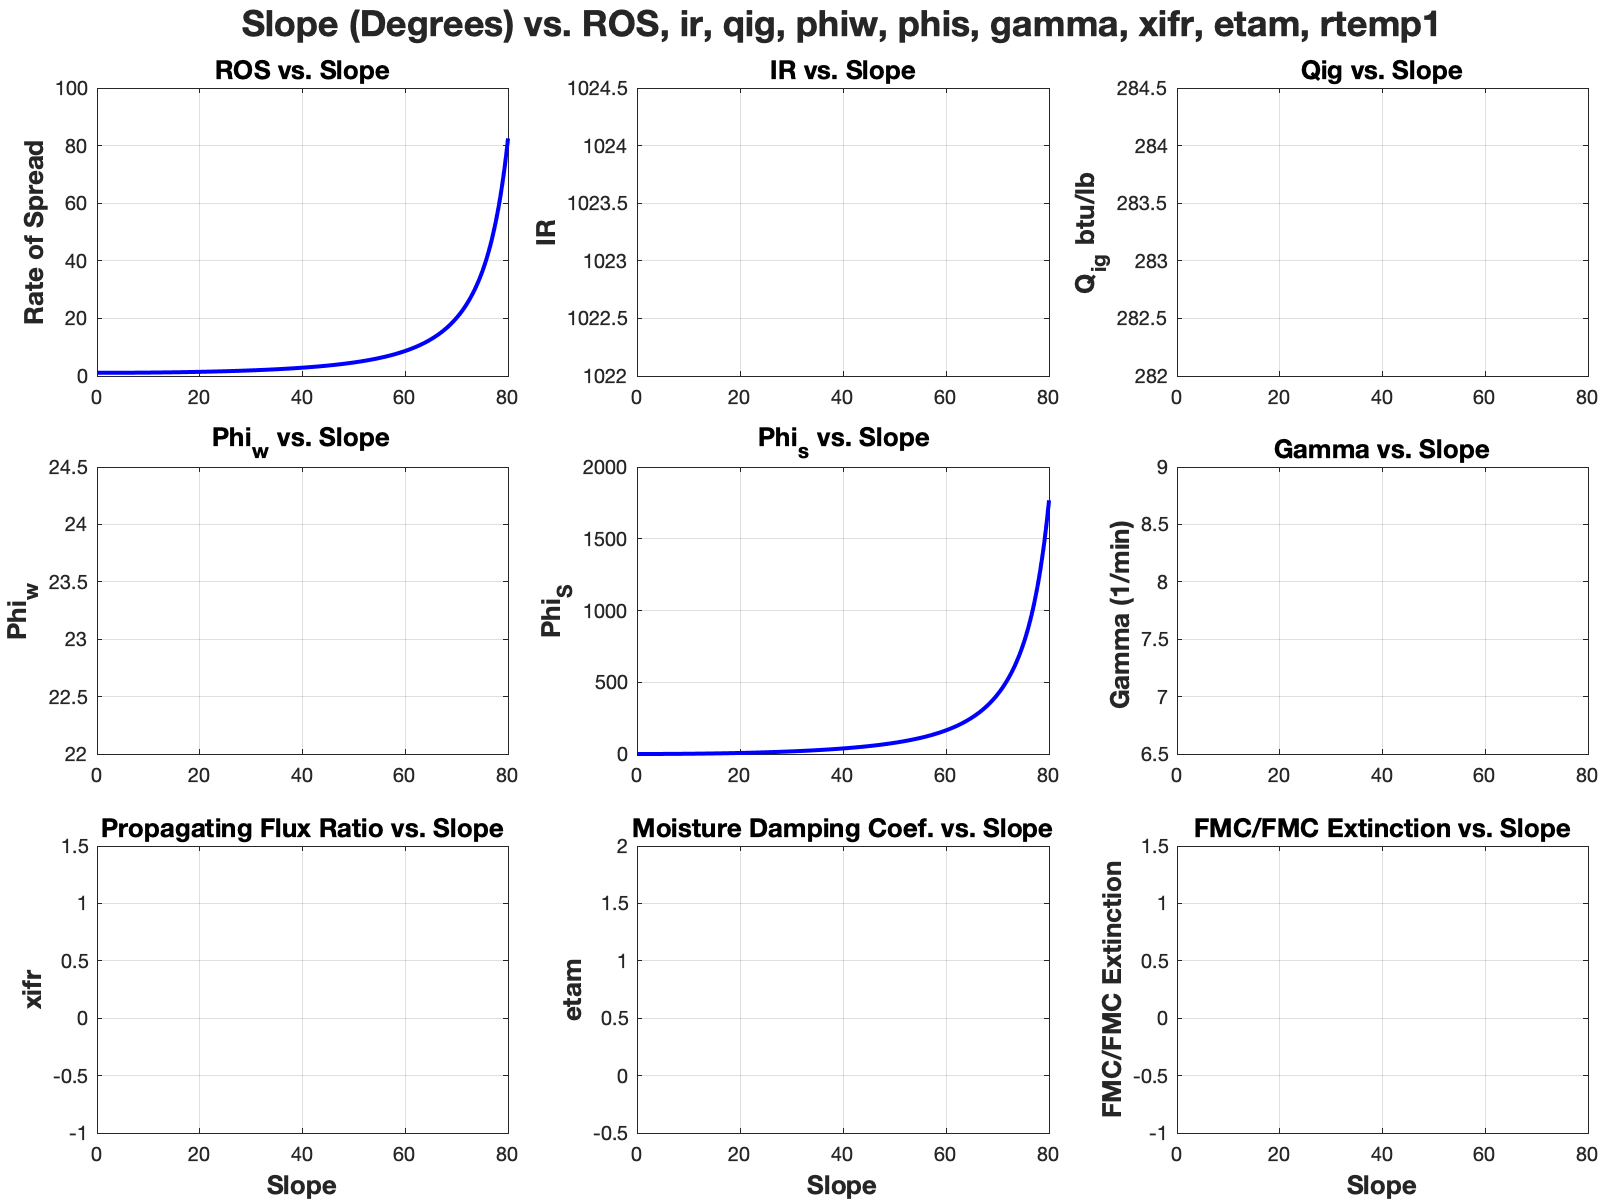
\includegraphics[width=1\linewidth]{/Users/jeremybenik/Research_Files/164/Assignments/draft/Images/Rothermel/slope_rothermel.png}
  \captionof{figure}{Rothermel Model}
  \label{fig:test1}
\end{minipage}%
\begin{minipage}{.5\textwidth}
  \centering
  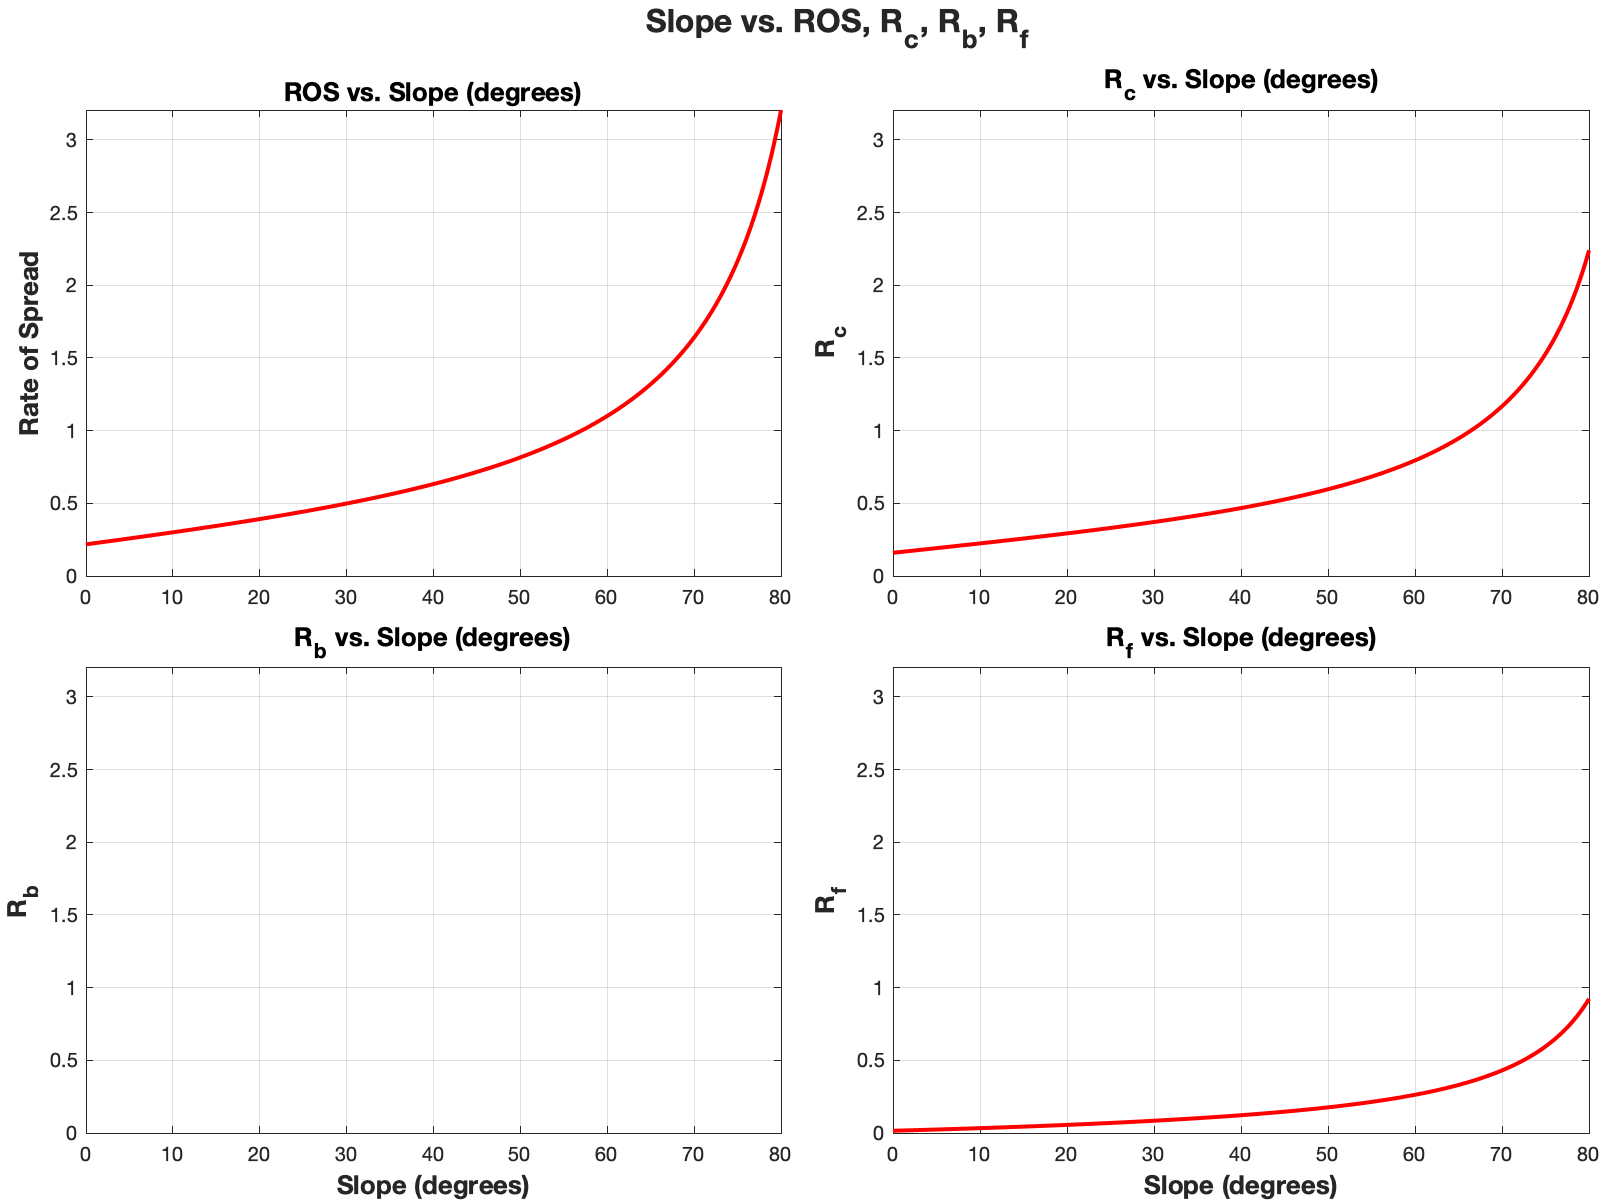
\includegraphics[width=1\linewidth]{/Users/jeremybenik/Research_Files/164/Assignments/draft/Images/Balbi/Slope.png}
  \captionof{figure}{Balbi Model}
  \label{fig:test2}
\end{minipage}
\end{figure}
\end{frame}


\begin{frame} {Comparisons between the models}
\framesubtitle{FMC Comparison}
\begin{figure}
\centering
\begin{minipage}{.5\textwidth}
  \centering
  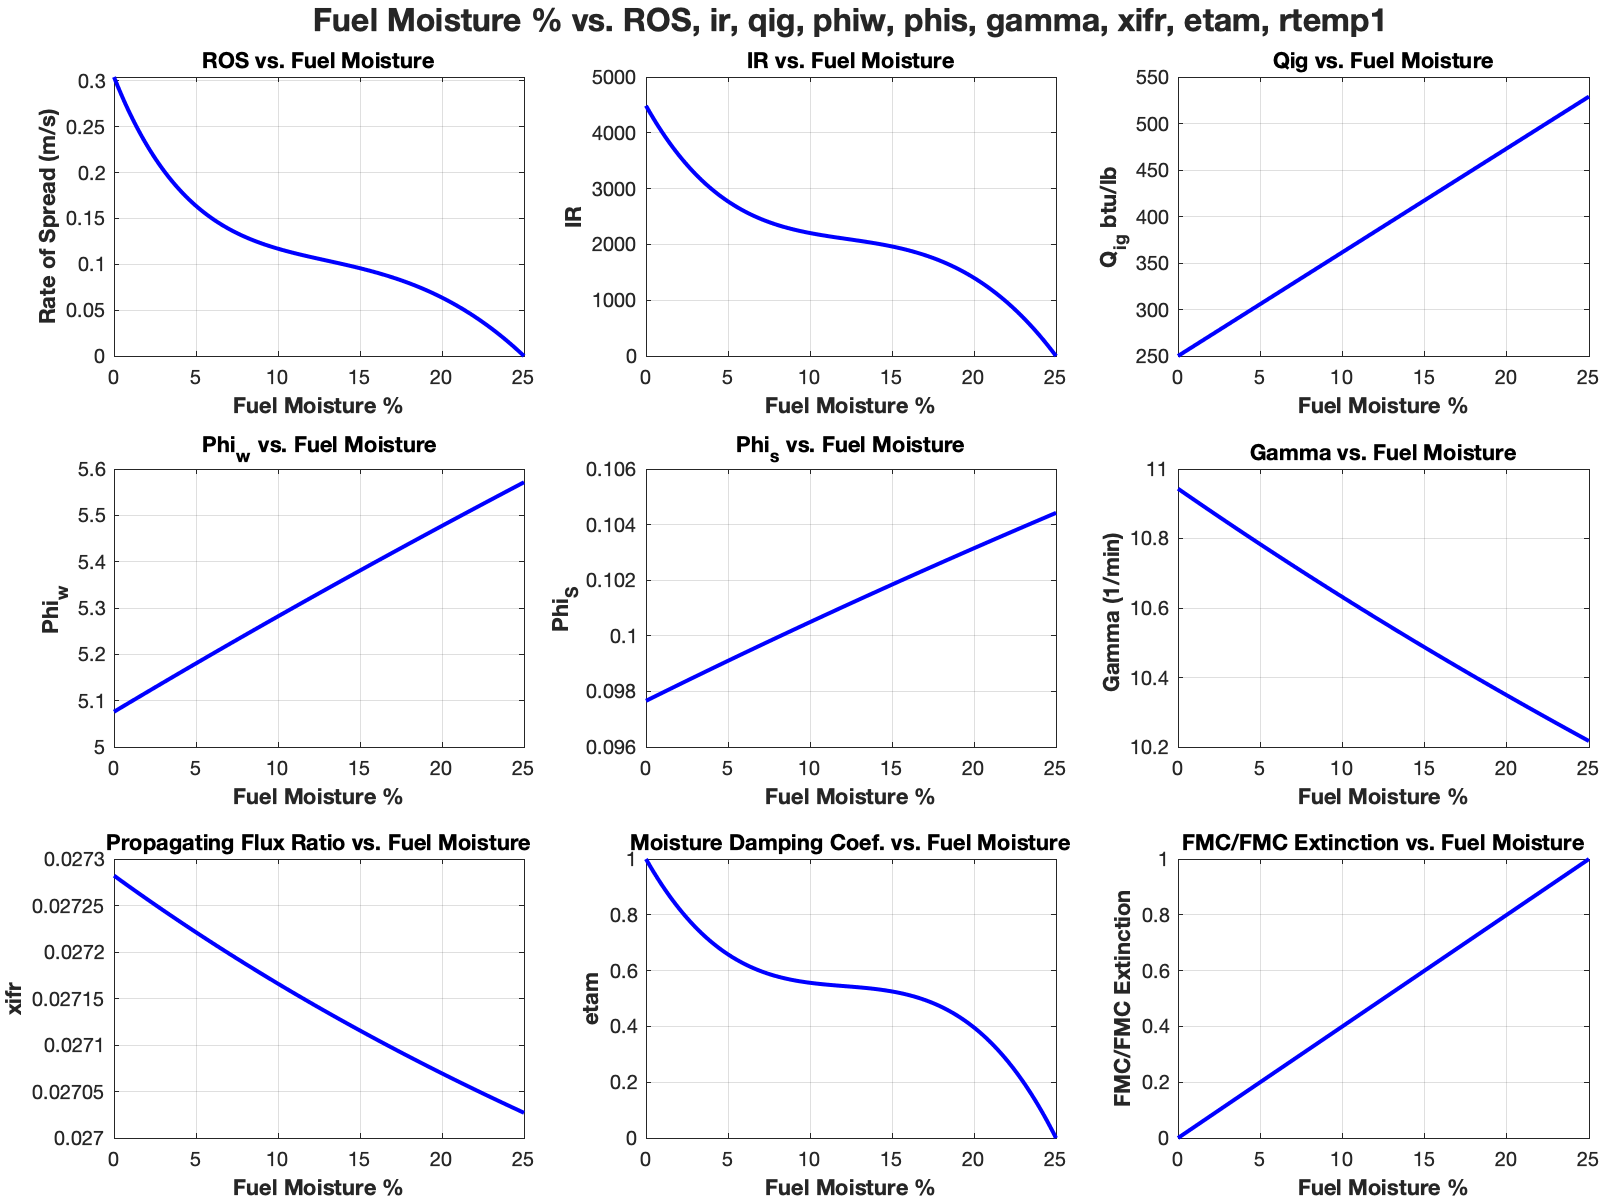
\includegraphics[width=1\linewidth]{/Users/jeremybenik/Research_Files/164/Assignments/draft/Images/Rothermel/FMC_rothermel.png}
  \captionof{figure}{Rothermel Model}
  \label{fig:test1}
\end{minipage}%
\begin{minipage}{.5\textwidth}
  \centering
  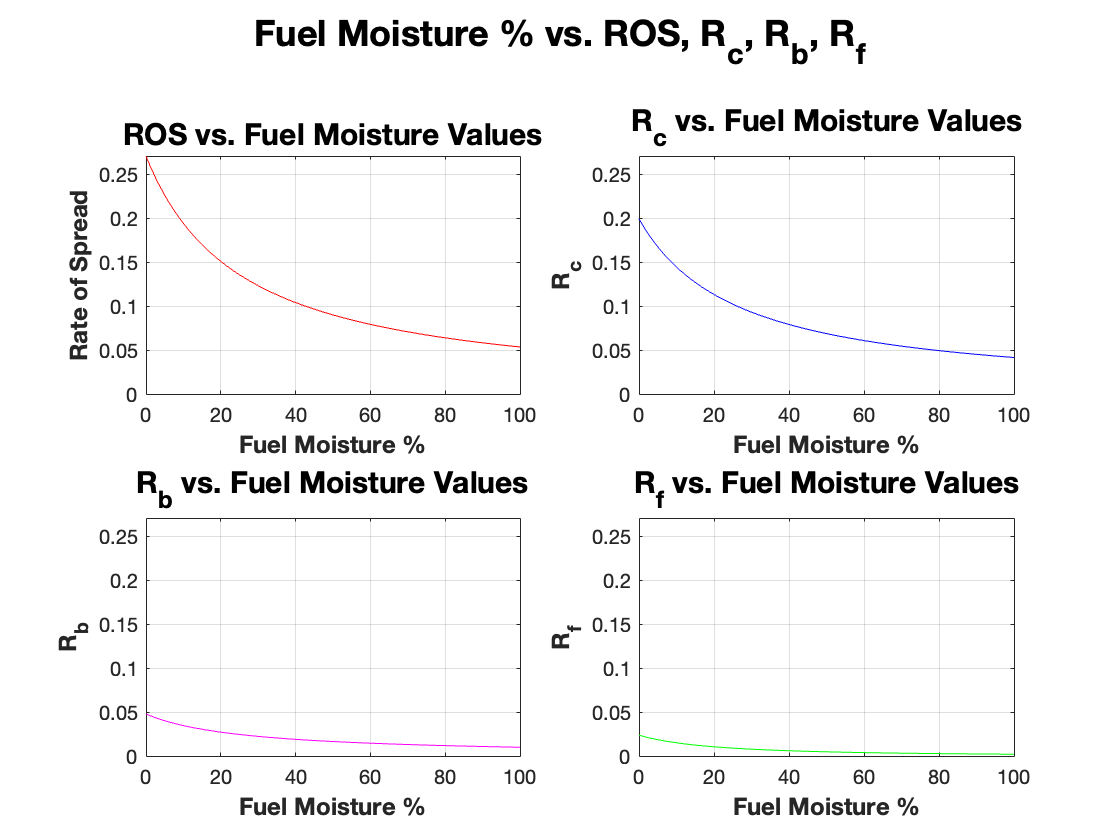
\includegraphics[width=1\linewidth]{/Users/jeremybenik/Research_Files/164/Assignments/draft/Images/Balbi/FMC_with_slope.png}
  \captionof{figure}{Balbi Model}
  \label{fig:test2}
\end{minipage}
\end{figure}
\end{frame}


\begin{frame} {Comparisons between the models}
\framesubtitle{FMC Rothermel}
\begin{figure}[h]
\centering
  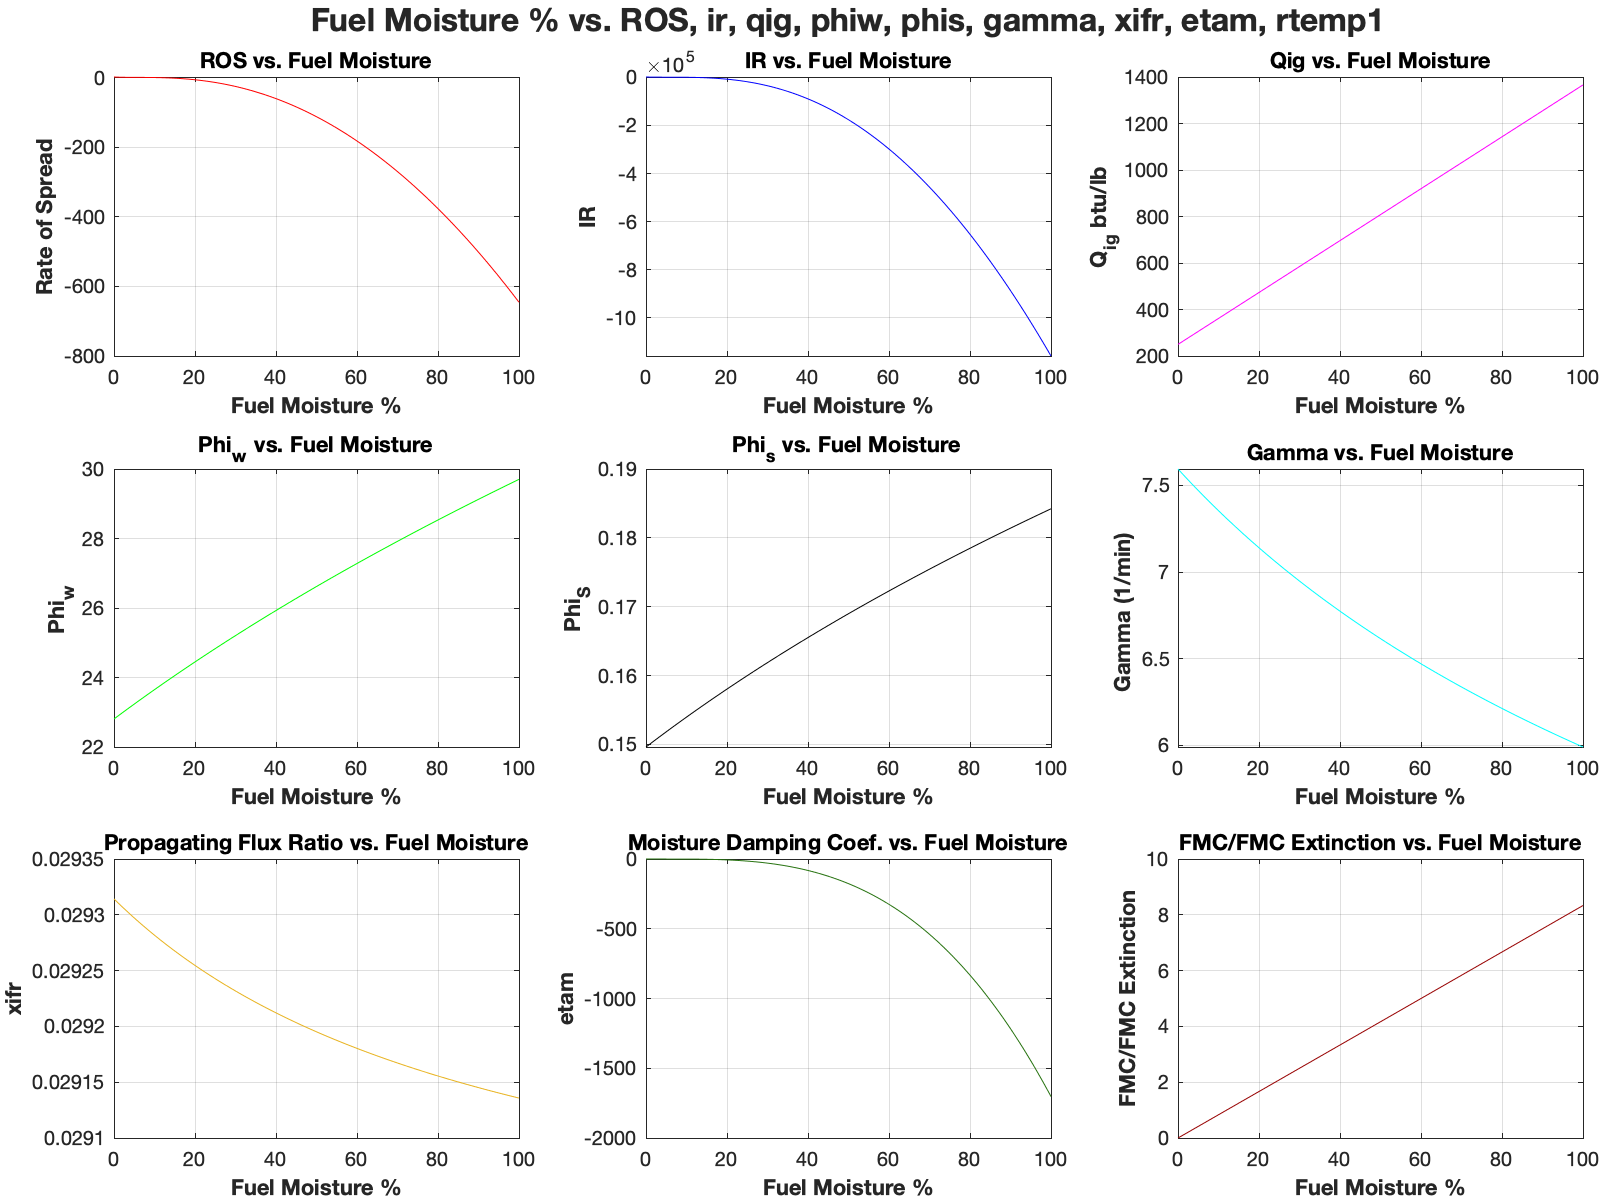
\includegraphics[scale = 0.15]{/Users/jeremybenik/Research_Files/164/Assignments/draft/Images/Rothermel/FMC_Rothermel_negative_vals.png}
  \caption{Rothermel model FMC without considering extinction FMC}
  \label{Balbi_flame_diagram}
\end{figure}
\end{frame}

\begin{frame} {Comparisons between the models}
\framesubtitle{Fuel Height Comparison}
\begin{figure}
\centering
\begin{minipage}{.5\textwidth}
  \centering
  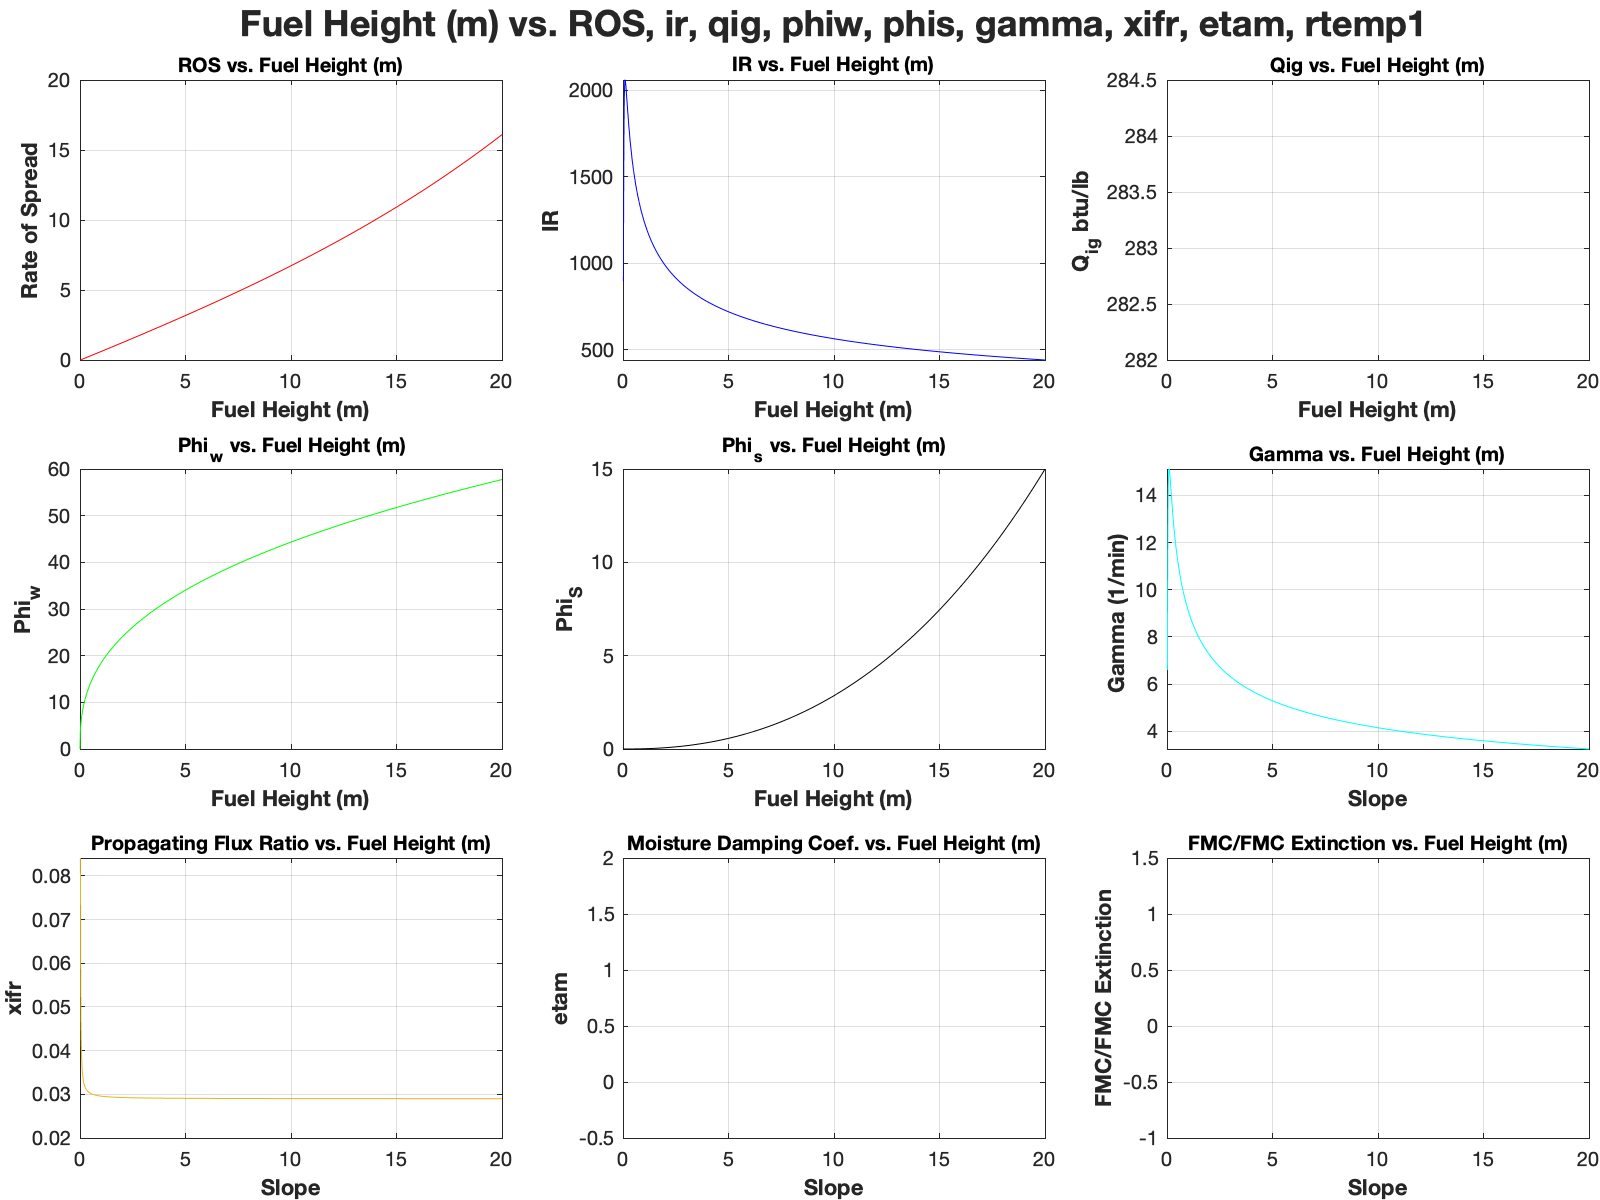
\includegraphics[width=1\linewidth]{/Users/jeremybenik/Research_Files/164/Assignments/draft/Images/Rothermel/fuel_height_rothermel.png}
  \captionof{figure}{Rothermel Model}
  \label{fig:test1}
\end{minipage}%
\begin{minipage}{.5\textwidth}
  \centering
  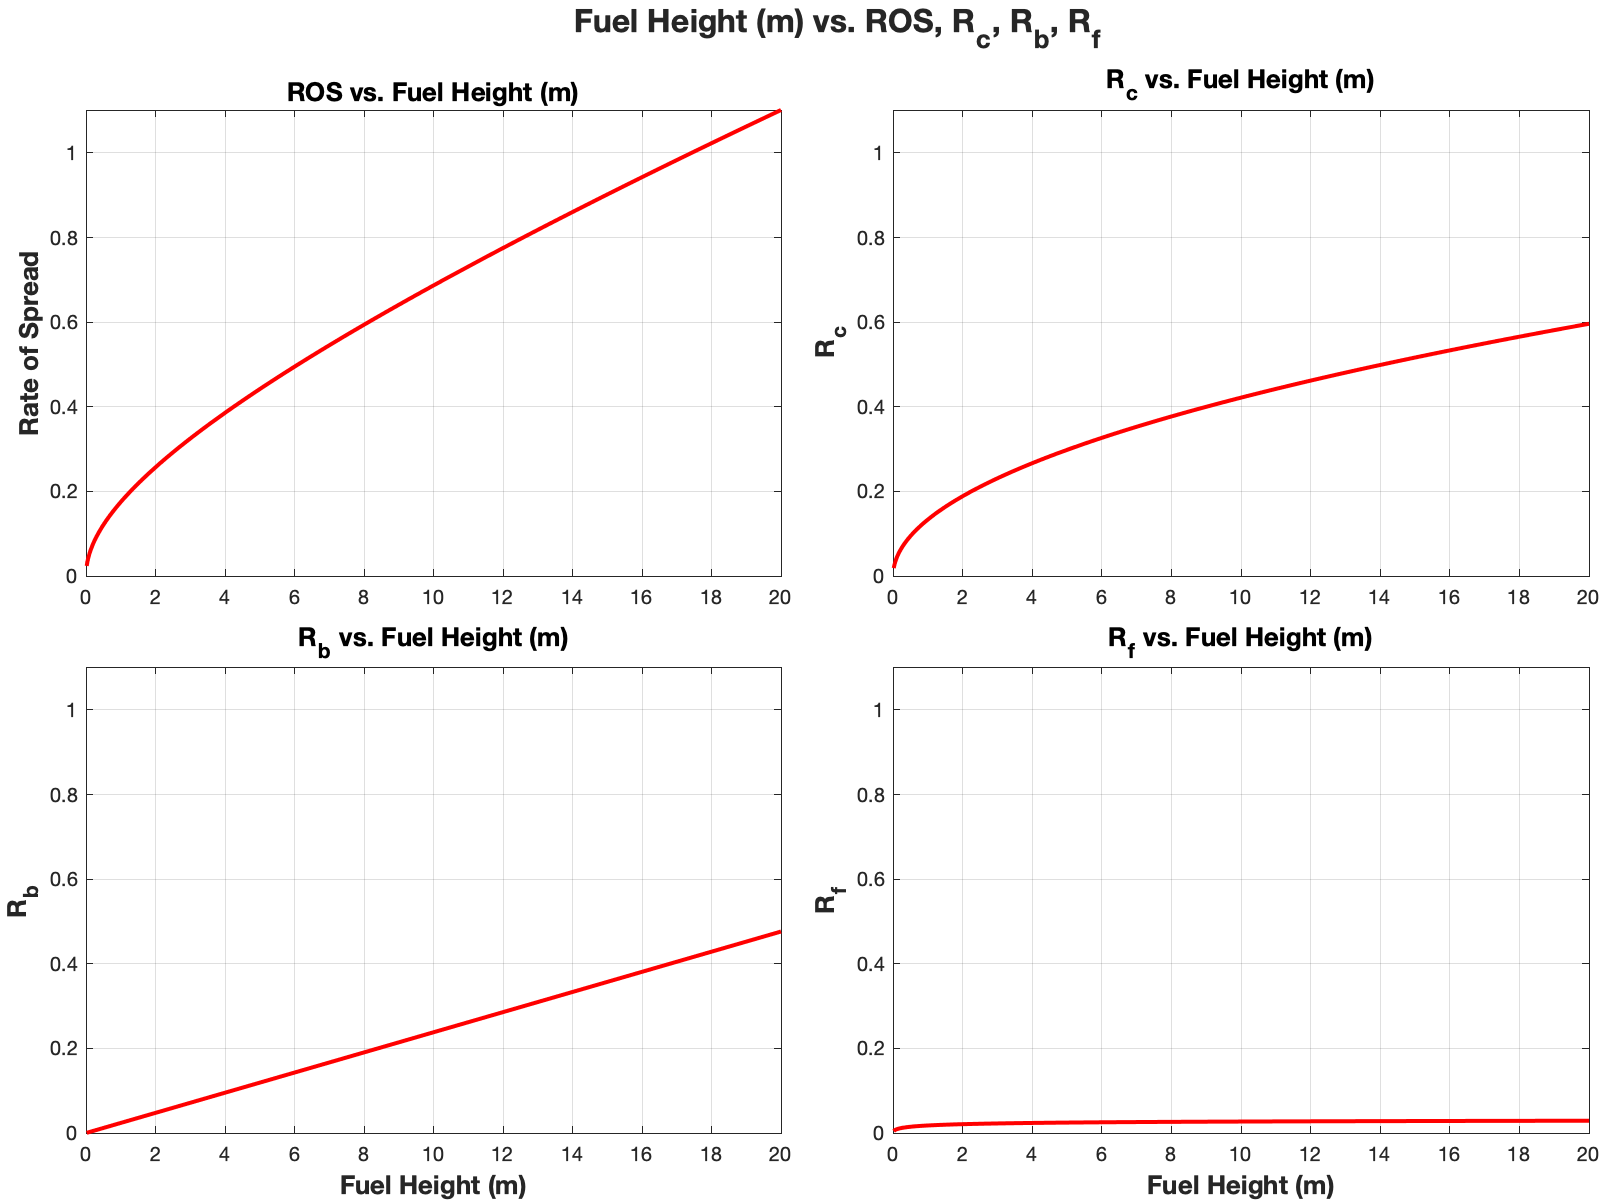
\includegraphics[width=1\linewidth]{/Users/jeremybenik/Research_Files/164/Assignments/draft/Images/Balbi/fuel_depth_m.png}
  \captionof{figure}{Balbi Model}
  \label{fig:test2}
\end{minipage}
\end{figure}
\end{frame}

\begin{frame} {Comparisons between the models}
\framesubtitle{SAVR Comparison}
\begin{figure}
\centering
\begin{minipage}{.5\textwidth}
  \centering
  \includegraphics[width=1\linewidth]{/Users/jeremybenik/Research_Files/164/Assignments/draft/Images/Rothermel/SAVR.png}
  \captionof{figure}{Rothermel Model}
  \label{fig:test1}
\end{minipage}%
\begin{minipage}{.5\textwidth}
  \centering
  \includegraphics[width=1\linewidth]{/Users/jeremybenik/Research_Files/164/Assignments/draft/Images/Balbi/SAVR.png}
  \captionof{figure}{Balbi Model}
  \label{fig:test2}
\end{minipage}
\end{figure}
\end{frame}


\begin{frame} {References}
\begin{figure}[h]
\centering
  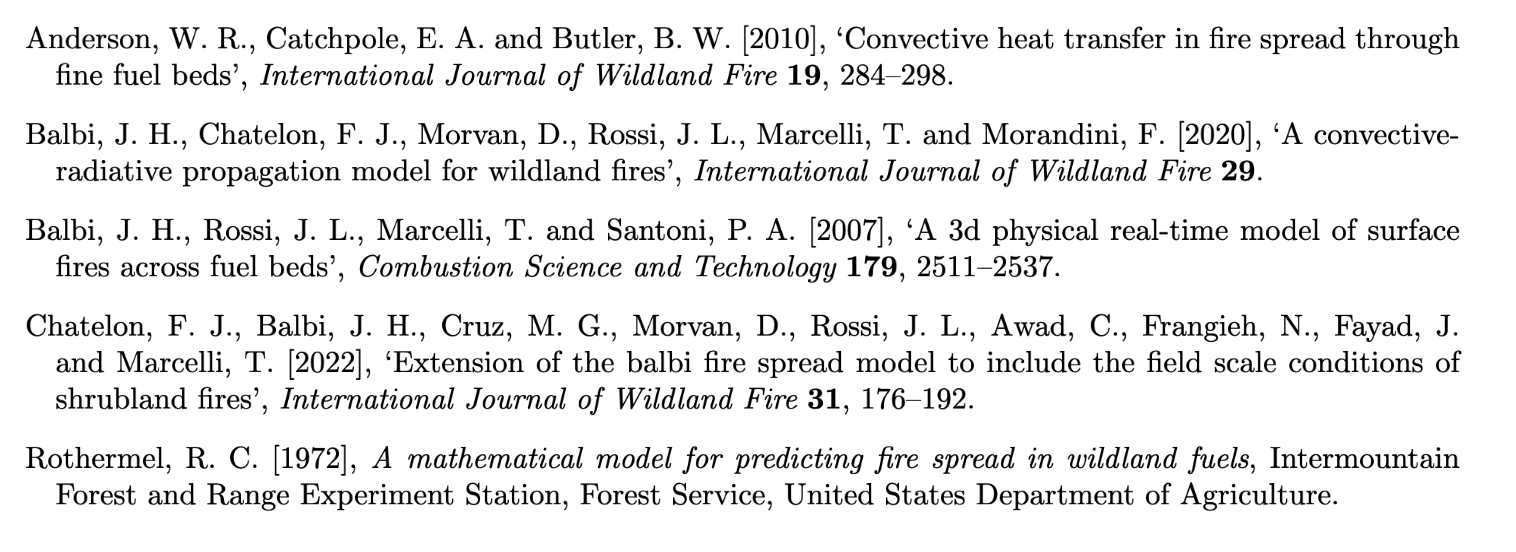
\includegraphics[scale = 0.4]{bib.png}
  \end{figure}
\end{frame}

\begin{frame} {Questions?}
\begin{center}
{\fontsize{40}{50}\selectfont Questions?}
\end{center}
\begin{itemize}
	\setlength{\itemsep}{10mm}
	\item Feel free to contact me with any further questions at: jeremy.benik@sjsu.edu
\end{itemize}
\end{frame}



\begin{frame} {Thank you}
\begin{center}
{\fontsize{40}{50}\selectfont Thank you!}
\end{center}
\begin{itemize}
	\item Here is a link to my codes if anyone wants to check them out
	\begin{itemize}
 	\item \url{https://github.com/Jeremy-Benik/164/tree/main/Assignments/Final_Drafts/Codes}
  	\end{itemize}
\end{itemize}
	
\end{frame}


\end{document}